% Asset ID: AS1CoordinateGeometryCirclesTikZ-002
% Purpose: Derive x^2 + y^2 = r^2 using Pythagoras.
\documentclass[tikz,border=8pt]{standalone}
\usetikzlibrary{calc,angles,quotes}
\begin{document}
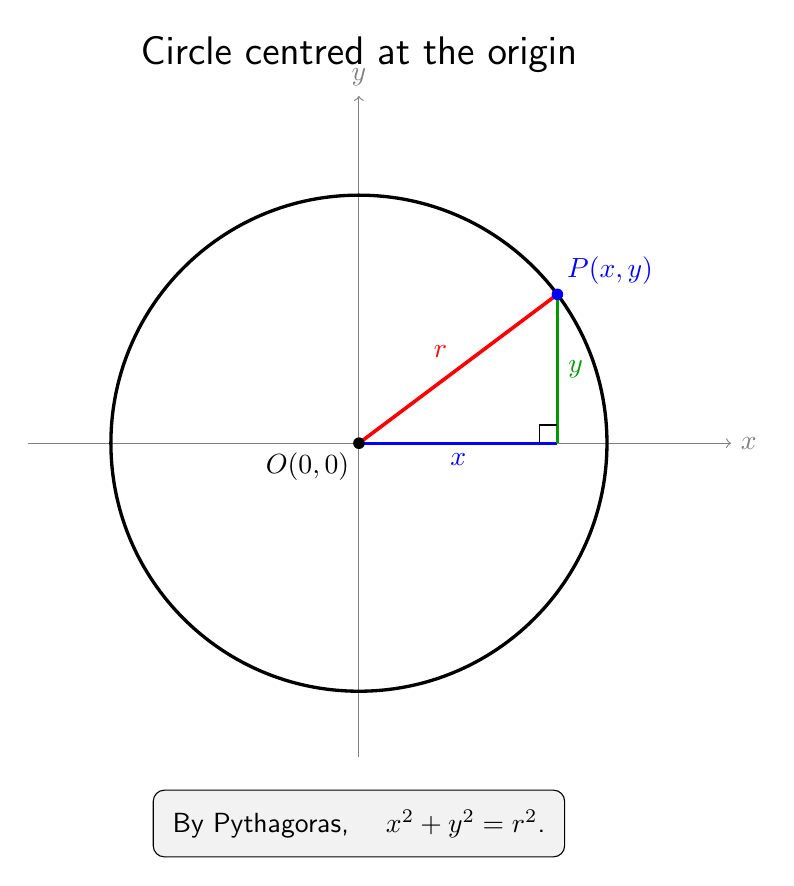
\begin{tikzpicture}[scale=1.05, font=\sffamily]
\draw[->, gray] (-4,0) -- (4.5,0) node[right] {$x$}; \draw[->, gray] (0,-3.8) -- (0,4.2) node[above] {$y$};
\coordinate (O) at (0,0); \draw[line width=1.2pt] (O) circle (3); \coordinate (P) at (2.4,1.8); \coordinate (Q) at (2.4,0);
\draw[line width=1.3pt, red] (O) -- (P) node[midway, above left] {$r$}; \draw[line width=1.2pt, blue] (O) -- (Q) node[midway, below] {$x$}; \draw[line width=1.2pt, green!60!black] (Q) -- (P) node[midway, right] {$y$};
\fill[black] (O) circle (2pt) node[below left] {$O(0,0)$}; \fill[blue] (P) circle (2pt) node[above right] {$P(x,y)$}; \draw (2.18,0) -- (2.18,0.22) -- (2.4,0.22);
\node[align=center] at (0,4.7) {\Large Circle centred at the origin};
\node[align=center, draw, rounded corners, fill=gray!10, inner sep=7pt] at (0,-4.6) {By Pythagoras, \quad $x^2+y^2=r^2$.};
\end{tikzpicture}\end{document}
